% TODO
\subsubsection{Modelo gráfico}
En la figura \ref{fig:SIR_devs_flattened} se observa en color azul los atómicos Fplus y Fminus asociados al flujo \textit{Succumbing}, mientras que en naranja se observan los atómicos Fplus y Fminus asociados al flujo \textit{Recovering}. En violeta se pueden ver las conexiones que representan de qué manera los diferentes atómicos correspondientes a cada uno de los flujos utilizan para realizar sus cálculos internos el output de \textit{InfectedIntegrator}, correspondiéndose cada una de estas flechas con una de las flechas del modelo gráfico mostrado en la figura \ref{fig:SIR_sd}. Como ya explicamos anteriormente, en este ejemplo sólo trabajaremos con la versión aplanada del modelo DEVS, para simplificar levemente el problema de traducción. 

Nuevamente, dejamos en rojo los atómicos que no tienen cabida en el modelo, pero que igualmente exponemos, para dejar explícito que esos atómicos podrían estar si hubiera un inflow/outflow que se les corresponda, pero que en este ejemplo no lo están.
\begin{figure}[!h]
\centering
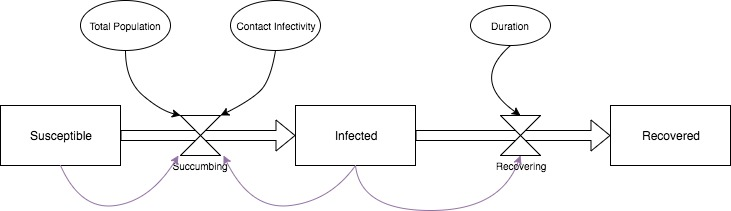
\includegraphics[scale=0.5]{imagenes/SIR_sd.jpg}
\caption{Modelo SIR expresado en System Dynamics en formato gráfico}
\label{fig:SIR_sd}
\end{figure}
\begin{figure}[!h]
\centering
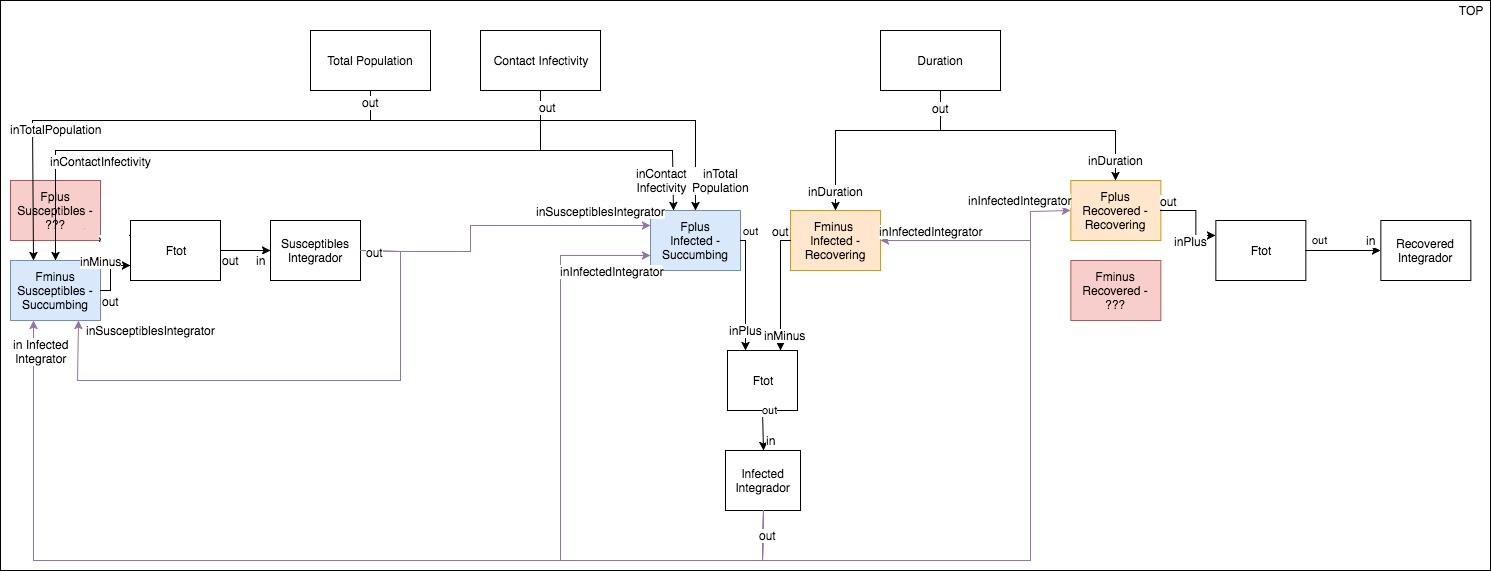
\includegraphics[scale=0.3]{imagenes/SIR_devs_flattened.jpg}
\caption{Modelo SIR expresado en DEVS en formato gráfico}
\label{fig:SIR_devs_flattened}
\end{figure}
\begin{figure}[!h]
\centering
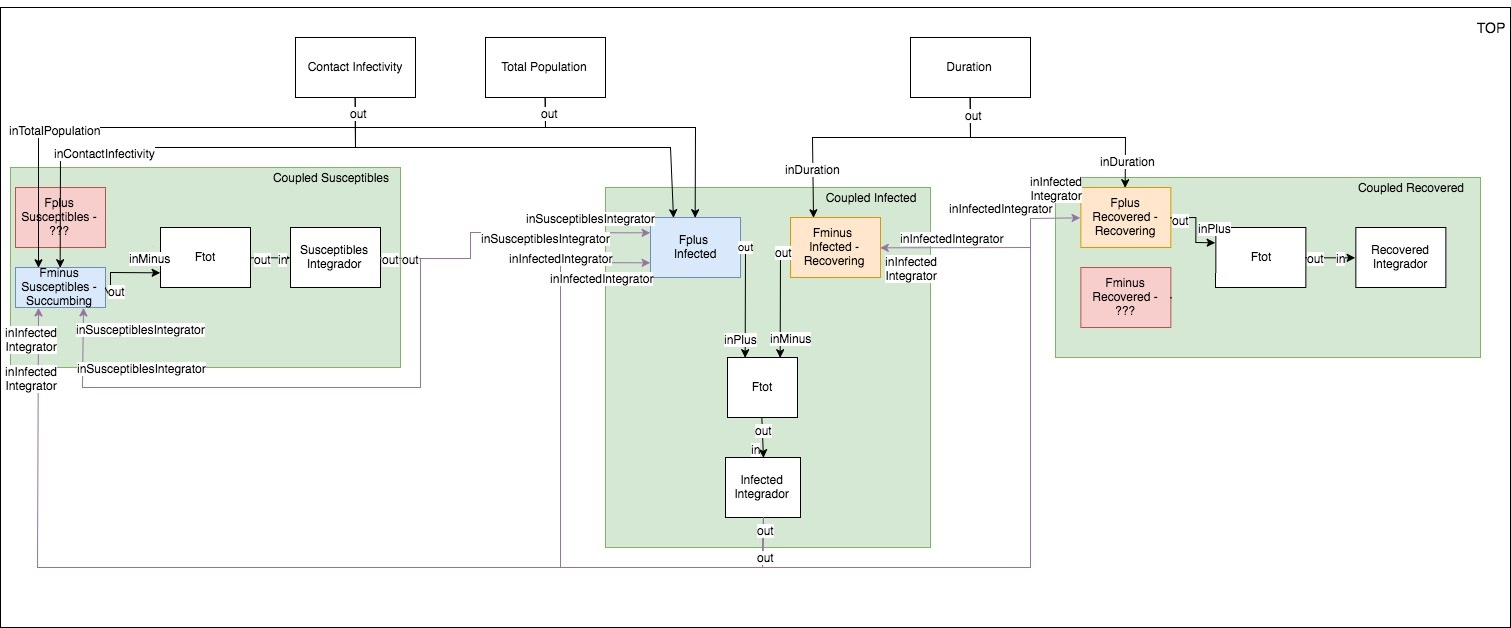
\includegraphics[scale=0.3]{imagenes/SIR_devs.jpg}
\caption{Modelo SIR expresado en DEVS en formato gráfico con varios niveles de acoplamiento}
\label{fig:SIR_devs}
\end{figure}
% TODO
\subsubsection{Modelo formal}
A continuación, exponemos formalmente los modelos atómicos utilizados en el acoplado Top, con la descripción de su comportamiento interno.
\begin{itemize}
\item \textbf{Cte} : $ totalPopulation, contactInfectivity, duration \rightarrow \langle X, S, Y, \delta_{int}, \delta_{ext}, \lambda, t_{a} \rangle$ \newline
$ X = \{ inValue \} $ \newline
$ S = \{ value \} $ \newline
$ Y = \{ out \} $ \newline
$ \delta_{int}(\langle value \rangle) = \emptyset $ \newline
$ \delta_{ext} (\langle value \rangle, e, x)= \{ value := x.value \} $ \newline
$ \lambda(\langle value \rangle, out) = value $ \newline
$ t_{a}(s) = \infty $

\item \textbf{Fminus} : $ fmSusceptiblesSuccumbing \rightarrow \langle X, S, Y, \delta_{int}, \delta_{ext}, \lambda, t_{a} \rangle$ \newline
$ X = \{ inTotalPopulation, inContactInfectivity, inInfectedIntegrator, inSuceptiblesIntegrator \} $ \newline
$ S = \{ totalPopulation, contactInfectivity, infectedIntegrator, suceptiblesIntegrator, isSetTotalPopulation, \newline isSetContactInfectivity, isSetInfectedIntegrator, isSetSuceptiblesIntegrator \} $ \newline
$ Y = \{ out \} $ \newline
$ \delta_{int}(s) = \emptyset $ \newline
$ \delta_{ext}(s, e, x) = \{
\\if (x.port = inTotalPopulation) totalPopulation := x.value; isSetTotalPopulation := true
\\if (x.port = inContactInfectivity) contactInfectivity := x.value; isSetContactInfectivity := true
\\if (x.port = inInfectedIntegrator) infectedIntegrator = x.value; \\isSetInfectedIntegrator := true 
\\if (x.port = inSuceptiblesIntegrator) suceptiblesIntegrator = x.value; \\isSetSuceptiblesIntegrator := true
\} $ \newline
$ \lambda(s, out) = if(todas \ las \ variables \ seteadas) \{ 
\\susceptiblesIntegrator*infectedIntegrator/totalPopulation*contactInfectivity\} \ else \ \emptyset$ \newline
$ t_{a} = \infty $ 

\item \textbf{Fplus} : $ fpInfectedSuccumbing \rightarrow \langle X, S, Y, \delta_{int}, \delta_{ext}, \lambda, t_{a} \rangle$ \newline
$ X = \{ inTotalPopulation, inContactInfectivity, inInfectedIntegrator, inSuceptiblesIntegrator \} $ \newline
$ S = \{ totalPopulation, contactInfectivity, infectedIntegrator, suceptiblesIntegrator, isSetTotalPopulation, \newline isSetContactInfectivity, isSetInfectedIntegrator, isSetSuceptiblesIntegrator \} $ \newline
$ Y = \{ out \} $ \newline
$ \delta_{int}(s) = \emptyset $ \newline
$ \delta_{ext}(s, e, x) = \{
\\if (x.port = inTotalPopulation) totalPopulation := x.value; isSetTotalPopulation := true
\\if (x.port = inContactInfectivity) contactInfectivity := x.value; isSetContactInfectivity := true
\\if (x.port = inInfectedIntegrator) infectedIntegrator = x.value; \\isSetInfectedIntegrator := true 
\\if (x.port = inSuceptiblesIntegrator) suceptiblesIntegrator = x.value; \\isSetSuceptiblesIntegrator := true
\} $ \newline
$ \lambda(s, out) = if(todas \ las \ variables \ seteadas) \{ 
\\susceptiblesIntegrator*infectedIntegrator/totalPopulation*contactInfectivity\} \ else \ \emptyset$ \newline
$ t_{a} = \infty $ 

\item \textbf{Fminus} : $ fmInfectedRecovering \rightarrow \langle X, S, Y, \delta_{int}, \delta_{ext}, \lambda, t_{a} \rangle$ \newline
$ X = \{ inDuration, inInfectedIntegrator \} $ \newline
$ S = \{ duration, infectedIntegrator, isSetDuration, isSetInfectedIntegrator \} $ \newline
$ Y = \{ out \} $ \newline
$ \delta_{int}(s) = \emptyset $ \newline
$ \delta_{ext}(s, e, x) = \{
\\if (x.port = inDuration) duration := x.value; isSetDuration := true
\\if (x.port = inInfectedIntegrator) infectedIntegrator = x.value; \\isSetInfectedIntegrator := true 
\} $ \newline
$ \lambda(s, out) = if(todas \ las \ variables \ seteadas) \{ 
\\infectedIntegrator/duration\} \ else \ \emptyset$ \newline
$ t_{a} = \infty $ 

\item \textbf{Fplus} : $ fpRecoveredRecovering \rightarrow \langle X, S, Y, \delta_{int}, \delta_{ext}, \lambda, t_{a} \rangle$ \newline
$ X = \{ inDuration, inInfectedIntegrator \} $ \newline
$ S = \{ duration, infectedIntegrator, isSetDuration, isSetInfectedIntegrator \} $ \newline
$ Y = \{ out \} $ \newline
$ \delta_{int}(s) = \emptyset $ \newline
$ \delta_{ext}(s, e, x) = \{
\\if (x.port = inDuration) duration := x.value; isSetDuration := true
\\if (x.port = inInfectedIntegrator) infectedIntegrator = x.value; \\isSetInfectedIntegrator := true 
\} $ \newline
$ \lambda(s, out) = if(todas \ las \ variables \ seteadas) \{ 
\\infectedIntegrator/duration\} \ else \ \emptyset$ \newline
$ t_{a} = \infty $

\item \textbf{Ftot} : $ ftSuceptibles, ftInfected, ftRecovered \rightarrow \langle X, S, Y, \delta_{int}, \delta_{ext}, \lambda, t_{a} \rangle$ \newline
$ X = \{ inMinus, inPlus \} $ \newline
$ S = \{ plus, minus \} $ \newline
$ Y = \{ out \} $ \newline
$ \delta_{int}(\langle plus, minus \rangle) = \emptyset $ \newline
$ \delta_{ext}(\langle plus, minus \rangle, e, x) = \{ 
\\if (x.port = inPlus) plus := x.value
\\if (x.port == inMinus) minus := x.value
\} $ \newline
$ \lambda(\langle plus, minus \rangle, out) = (plus - minus) $ \newline
$ t_{a} = \infty $ 


\item \textbf{QSS1} : $ susceptiblesIntegrator, infectedIntegrator, recoveredIntegrator  \rightarrow \langle X, S, Y, \delta_{int}, \delta_{ext}, \lambda, t_{a} \rangle$ \newline
$ X = \{ in \} $ \newline
$ S = \{ ? \} $ \newline
$ Y = \{ out \} $ \newline
$ \delta_{int}(s) = \{ ? \} $ \newline
$ \delta_{ext}(s, e, x) = \{ ? \} $ \newline
$ \lambda(s) = ? $ \newline
$ t_{a} = \{ ? \} $ 
\end{itemize}

El acoplado que utiliza los atómicos expuestos más arriba es:

% TODO modificar el acoplado para darle forma al acoplado de SIR
\begin{itemize}
	\item $ Top \rightarrow \langle X, Y, \{ M_{1}, M_{2}, M_{3}, M_{4}, M_{5} \}, C_{xx}, C_{yx}, C_{yy}, Select \rangle$ \newline
	$ X = \{ \} $ \newline
	$ Y = \{ \} $ \newline
	$ M_{1} = totalPopulation $ \newline
	$ M_{2} = contactInfectivity $ \newline
	$ M_{3} = duration $ \newline
	$ M_{4} = fmSusceptiblesSuccumbing $ \newline
	$ M_{5} = ftSuceptibles  $ \newline
	$ M_{6} = susceptiblesIntegrator  $ \newline
	$ M_{7} = fpInfectedSuccumbing $ \newline
	$ M_{8} = fmInfectedRecovering  $ \newline
	$ M_{9} = ftInfected  $ \newline
	$ M_{10} = infectedIntegrator  $ \newline
	$ M_{11} = fpRecoveredRecovering  $ \newline
	$ M_{12} = ftRecovered  $ \newline
	$ M_{13} = recoveredIntegrator  $ \newline
	$ C_{xx} = $ \{ \} \newline
	$ C_{yx} = \{ (M_{1}.!out, M_{4}.?inTotalPopulation), (M_{1}.!out, M_{5}.?inTotalPopulation), \\
	(M_{2}.!out, M_{4}.?inContactInfectivity), (M_{2}.!out, M_{5}.?inContactInfectivity), \\
	(M_{3}.!out, M_{6}.?inDuration), (M_{3}.!out, M_{7}.?inDuration), \\
	(M_{4}.!out, M_{5}.?inMinus), (M_{5}.!out, M_{6}.?in), \\
	(M_{6}.!out, M_{4}.?inSusceptiblesIntegrator), (M_{6}.!out, M_{7}.?inSuceptiblesIntegrator), \\
	(M_{7}.!out, M_{9}.?inPlus), (M_{8}.!out, M_{9}.?inMinus), \\
	(M_{9}.!out, M_{10}.?in), (M_{10}.!out, M_{4}.?inInfectedIntegrator), \\
	(M_{10}.!out, M_{7}.?inInfectedIntegrator), (M_{10}.!out, M_{8}.?inInfectedIntegrator), \\
	(M_{10}.!out, M_{11}.?inInfectedIntegrator), (M_{11}.!out, M_{12}.?inPlus), \\
	(M_{12}.!out, M_{13}.?in)  \} $ \newline
	$ C_{yy} = \{ \} $ \newline
\end{itemize}

\subsubsection{Generación de modelo ejecutable en CD++}
